\documentclass[10pt,journal]{IEEEtran}
\usepackage[T1]{fontenc}
\usepackage{amsmath,amssymb,amsthm,graphicx,booktabs,array,url}
\usepackage{newtxtext,newtxmath}
\usepackage{microtype}
\usepackage{cite}
\usepackage[hidelinks]{hyperref}
\newtheorem{theorem}{Theorem}
\newtheorem{proposition}{Proposition}
\newtheorem{lemma}{Lemma}
\newtheorem{corollary}{Corollary}
\theoremstyle{remark}
\newtheorem{remark}{Remark}
% Auto-generated; do not edit by hand.
\newcommand{\CTwoWins}{11}
\newcommand{\CTwoLosses}{8}
\newcommand{\CTwoCases}{20}
\newcommand{\CTwoRank}{0.74}
\newcommand{\CTwoMedian}{+4.1}
\newcommand{\CTwoFixedWins}{3}
\newcommand{\CTwoFixedLosses}{9}
\newcommand{\CTwoGateWins}{14}
\newcommand{\CTwoGateLosses}{6}
\newcommand{\CTwoVoneWins}{8}
\newcommand{\CTwoVoneLosses}{12}
\newcommand{\CTwoVoneRank}{0.26}
\newcommand{\CThreeZero}{21}
\newcommand{\CThreeZeroMax}{43}
\newcommand{\CThreeFive}{2.3}
\newcommand{\CThreeIBM}{0.004}
\newcommand{\CFourRobust}{1.000}
\newcommand{\CFourPlugin}{0.502}
\newcommand{\CFourInside}{0}
\newcommand{\CFourInsideCases}{30}
\newcommand{\CFourPlainInside}{0}
\newcommand{\CFourPlainOutside}{6}
\newcommand{\CFourOutsideCases}{12}
\newcommand{\CFourExtendedOutside}{0}
\newcommand{\CFourTrials}{1200}
\newcommand{\CFourSlack}{23}
\newcommand{\CFiveViolations}{3}
\newcommand{\CFiveFalse}{2}
\newcommand{\CFiveCases}{6}
\newcommand{\CSixTrials}{300}
\newcommand{\CSixViolations}{0}
\newcommand{\CEightGates}{133{,}160}
\newcommand{\CEightTime}{1087.7}
\newcommand{\CEightGap}{6e-02}


\title{Geometric Programming for Quantum Resource Allocation:\\
Globally Optimal Co-Design of Gate Timing, Dynamical Decoupling, and Error-Mitigation Budgets}
\author{Youssef Ahmed Ramadan%
\thanks{Y. A. Ramadan is with the Department of Artificial Intelligence Engineering, School of Engineering,
University of Science and Technology at Zewail City, Giza, Egypt (e-mail: p-youssef.ramdan@zewailcity.edu.eg).}}

\begin{document}
\maketitle

\begin{abstract}
Compilers for noisy quantum processors must decide how long each gate takes, where idle time falls, how
idle qubits are dynamically decoupled, and how many shots error mitigation needs. We show that, under
Markovian Pauli--Lindblad noise whose rates depend on these resources by power laws, the quantities a
compiler cares about---log-fidelity of tracked observables, the sampling overhead of probabilistic error
cancellation (PEC), estimator variance, and total QPU time---are posynomials or exponentials of posynomials.
Their joint allocation is therefore a geometric program, or convex in logarithmic coordinates, and is solved
to global optimality with a dual certificate. Five results follow. (i)~Gate durations, idle placement and
dynamical-decoupling pulse counts are \emph{jointly convex} through a perspective structure, with a closed-form
optimal pulse count and a drive-versus-idle threshold that says exactly when a gate should be stretched.
(ii)~The QPU time of a PEC-mitigated estimate has the closed-form optimum
$\tau_j^\star=\sqrt{a_j/(g_j+p_j/4(M+t_{\rm rep}))}$, where $p_j$ is a critical-path flow. (iii)~An
ellipsoidal robust counterpart remains an exact geometric program and carries a calibration-coverage
certificate, and baseline-dominance constraints guarantee that the optimised schedule never loses to the
compiler's default on any error law in a declared convex hull. (iv)~Anisotropic, state-aware hazards remain
posynomial, and isotropic models provably cannot represent basis-dependent rankings of the kind measured on
IBM Heron. (v)~Discrete pulse-library selection is strongly NP-hard, while log-grid rounding of the relaxation
is a $(q,q)$-bicriteria approximation. In independent time-correlated noise simulations with models fitted only
from spectroscopy, joint timing and decoupling beats the best of ASAP, ALAP, ALAP+XX and ALAP+XY4 in
\CTwoWins{} of \CTwoCases{} circuit--noise cases and loses in \CTwoLosses{} (median change \CTwoMedian$\times10^{-4}$).
The gains rely on duration control; with native fixed durations the method rarely beats the best standard
schedule, and low-frequency noise shared across idle windows remains its main failure mode. Runtime-optimal PEC reduces modelled
QPU time by a median of \CThreeZero\% without repetition overhead, but by only \CThreeIBM\% at IBM's default
repetition delay, as the theory predicts. Robust certificates reach a pooled empirical coverage of
\CFourRobust{} at a 0.95 target, versus \CFourPlugin{} for plug-in predictions. On IBM Heron, in a pre-registered test and replication using about one minute of free-tier
QPU time, the model predicted the ranking of five decoupling policies. The GP schedule beat the best standard
sequence (XY4) by 2.2 percentage points in all-qubit return probability (pooled 95\% interval 1.4--2.9), and it
correctly left a qubit undecoupled where decoupling hurt.
\end{abstract}

\begin{IEEEkeywords}
Quantum compilation, geometric programming, convex optimization, dynamical decoupling, error mitigation,
robust optimization, scheduling.
\end{IEEEkeywords}

\section{Introduction}
Quantum compilers increasingly make physical, not only logical, decisions: which pulse implements a gate,
when each gate starts, and how idle intervals are protected~\cite{murali2019,murali2020,earnest2021,lussi2025}.
These decisions trade drive-induced error against decoherence, idle dephasing against pulse errors, and
circuit latency against the shot budget of error mitigation~\cite{temme2017,vandenberg2023}. They are usually
taken by separate heuristics: an ASAP or ALAP scheduler, then a dynamical-decoupling (DD) pass that inserts a
fixed sequence wherever it fits~\cite{ezzell2023,das2021,ravi2022}.

This paper argues that a single mathematical object governs all of them. Under Markovian Pauli--Lindblad
noise, a stabilizer expectation decays as the exponential of a sum of Pauli intensities, and the PEC overhead
is the exponential of their total. If each intensity is a posynomial in the physical resources, every quantity
of interest is log-posynomial. Geometric programming (GP)~\cite{boyd2007} is the natural language, and it brings
global optimality, duality, sensitivity and robust counterparts with it. Earlier versions of this work used
GP only for gate durations on a fixed circuit, and their simulations showed little benefit~\cite{ramadan2026}.
Here we identify the decisions where the structure pays off and characterise exactly when it does not.

\paragraph*{Contributions}
\begin{enumerate}
\item A catalogue theorem (Theorem~\ref{thm:c1}) placing observable constraints, PEC overhead, estimator
variance and QPU time in one log-convex class.
\item Joint convexity of gate duration, idle placement and DD pulse counts under power-law dephasing spectra
(Theorem~\ref{thm:c2}), with a closed-form pulse count and a drive-versus-idle threshold
(Corollaries~\ref{cor:n}--\ref{cor:threshold}). Idle-aware timing is convex but not a GP (Remark~\ref{rem:notgp}).
\item The closed-form runtime-optimal schedule for PEC-mitigated estimation (Theorem~\ref{thm:c3}) and the
corollary that it reduces to error-optimal durations when repetition overhead dominates.
\item Certified robustness: an exact-GP ellipsoidal counterpart with a calibration-coverage guarantee
(Theorem~\ref{thm:c4}) and baseline dominance on a declared law hull (Theorem~\ref{thm:dom}).
\item Anisotropic and state-aware constraints (Propositions~\ref{prop:iso}--\ref{prop:state}), including a proof
that isotropic noise forces basis-independent rankings.
\item Strong NP-hardness of discrete library selection and a $(q,q)$-bicriteria rounding guarantee
(Theorems~\ref{thm:hard}--\ref{thm:bicriteria}); log-log convexity of the latency--fidelity frontier with a dual
``fidelity price'' (Proposition~\ref{prop:frontier}).
\item Open-source implementations, an independent time-correlated noise simulator, and a pre-registered
minimal-cost IBM protocol.
\end{enumerate}
Evidence comes from independent simulation and from a pre-registered hardware test with replication on IBM
Heron. The declared models and their limits are stated in Section~\ref{sec:limits}.

\section{Related work}
Time--cost trade-offs on DAGs date to Kelley and Fulkerson~\cite{kelley1961,fulkerson1961}; geometric programming
was developed for circuit sizing~\cite{boyd2005,boyd2007}, and the discrete time--cost problem is strongly
NP-hard~\cite{de1997} with known bicriteria approximations~\cite{skutella1998}. Duration-aware quantum
scheduling assigns fast pulses to critical paths and robust pulses to slack~\cite{lussi2025}. Filter-function
theory relates DD sequences to dephasing spectra~\cite{uhrig2007,cywinski2008,biercuk2011}; compiler work selects
DD per qubit adaptively~\cite{das2021} or variationally~\cite{ravi2022}, and a performance survey compares
sequences on superconducting hardware~\cite{ezzell2023}. PEC and its sparse Pauli--Lindblad implementation are
due to~\cite{temme2017,vandenberg2023}. To our knowledge no prior work proves joint convexity of timing and DD
allocation, or derives the runtime-optimal schedule for mitigated estimation.

\section{Model and preliminaries}\label{sec:model}
A circuit has timed gates $j=1,\dots,m$ with durations $\tau_j\in[\ell_j,u_j]$ and dependency DAG $\mathcal D$;
$M(\tau)$ is the longest path length. Gate $j$ is followed by a Pauli--Lindblad channel with per-Pauli
intensities $\lambda_{jP}(\tau_j)=a_{jP}\tau_j^{-p}+g_{jP}\tau_j$ and total $\lambda_j=\sum_P\lambda_{jP}$.
The following are known and are used without claim of novelty: convexity and GP form of
$\sum_j\lambda_j+bM$~\cite{boyd2005,boyd2007}; the path-flow minimax dual and its Frank--Wolfe
solution~\cite{kelley1961,fulkerson1961,jaggi2013}; and exact Pauli decay of stabilizer
expectations~\cite{vandenberg2023}.

\section{Theory}\label{sec:theory}
Full proofs are in the Appendix and in the repository (\texttt{docs/THEORY.md}).

\subsection{A log-posynomial catalogue}
\begin{theorem}[Catalogue]\label{thm:c1}
Let the intensities be posynomials in resources $x>0$. For a Clifford circuit with stabilizer generators $S_k$,
(1) $\langle S_k\rangle=\exp(-2\sum_j\sum_{P\in\mathcal A_{kj}}\lambda_{jP}(x))$, so $\langle S_k\rangle\ge t_k$
is a posynomial constraint; (2) PEC overhead is $\gamma=\exp(2\sum_{j,P}\lambda_{jP})$ and the PEC estimator
of a $\pm1$ observable has variance $\gamma^2-\langle O\rangle^2$; (3) $\log\gamma$ and $\log(\gamma^2/s)$
are convex in $\log x$.
\end{theorem}

\subsection{Joint timing and dynamical decoupling}
Idle windows lie between consecutive gates on a qubit and from a qubit's last gate to $M$; their widths
$w_k$ are affine in start times and durations. A window with $n_k$ refocusing pulses on qubit $q$ has hazard
\begin{equation}\label{eq:window}
h_q(w,n)=c_q\,w^{1+\beta_q}(n+1)^{-\beta_q}+\eta_q w+\epsilon_q n,\qquad n\tau_\pi\le w,
\end{equation}
which interpolates free induction ($n=0$) and the CPMG scaling $w^{1+\beta}n^{-\beta}$ under a
$\omega^{-\beta}$ spectrum~\cite{cywinski2008}.
\begin{theorem}[Joint convexity]\label{thm:c2}
Minimising $\sum_j(a_j/\tau_j+g_j\tau_j)+\sum_k h_{q(k)}(w_k,n_k)$ over durations, start times, makespan
$M\le D$ and real $n\ge0$ is a convex program whose value lower-bounds every integer DD assignment.
\end{theorem}
\begin{proof}[Proof sketch]
$w^{1+\beta}(n+1)^{-\beta}$ is the perspective of $x\mapsto x^{1+\beta}$ at $(w,n+1)$, hence jointly convex,
and $w$ is affine in the decision variables.
\end{proof}
\begin{corollary}[Pulse count]\label{cor:n}
For fixed $w$ and $\beta>0$, $n^\star+1=\max\{1,(\beta c\,w^{1+\beta}/\epsilon)^{1/(1+\beta)}\}$, capped by
$w/\tau_\pi$; the best even count is a neighbour of $n^\star$.
\end{corollary}
\begin{corollary}[Drive-versus-idle threshold]\label{cor:threshold}
Under white idle noise of total rate $\bar\eta_j$ on the qubits of gate $j$, if lengthening $\tau_j$ shortens
adjacent windows one-for-one, then $\tau_j^\star=\mathrm{clip}(\sqrt{a_j/(g_j-\bar\eta_j)})$ when
$g_j>\bar\eta_j$, and $\tau_j$ fills all available slack otherwise.
\end{corollary}
\begin{remark}\label{rem:notgp}
Idle time $M-\sum\tau$ carries a negative coefficient on $\tau$, so idle-aware timing is convex but not a GP in
$(\tau,M)$; for fixed windows it is an exact GP.
\end{remark}
\begin{proposition}[State-aware relaxation]\label{prop:state}
For Clifford, or small, circuits the ideal excited population $p_1$ of each idle window is computable, since
gates on other qubits do not change a qubit's reduced state. Weighting amplitude-damping exposure by $p_1$
(or by $1/2$ under an even CPMG block) adds nonnegative linear terms and preserves Theorem~\ref{thm:c2}; using
$\min(p_1,1/2)$ in the relaxation keeps it a valid lower bound.
\end{proposition}

\subsection{Runtime-optimal error mitigation}
\begin{theorem}[Runtime optimum]\label{thm:c3}
With $\Lambda=\sum_j(a_j/\tau_j+g_j\tau_j)$, the PEC QPU time
$T(\tau)=\epsilon^{-2}e^{4\Lambda(\tau)}(M(\tau)+t_{\rm rep})$ is log-convex in $\log\tau$, and every interior
optimal duration satisfies $\tau_j^\star=\sqrt{a_j/(g_j+p_j/(4(M^\star+t_{\rm rep})))}$ with
$p\in\partial M(\tau^\star)$, the convex hull of critical-path incidence vectors.
\end{theorem}
\begin{corollary}\label{cor:trep}
As $t_{\rm rep}\to\infty$, $\tau_j^\star\to\sqrt{a_j/g_j}$: when repetition overhead dominates, minimising QPU
time reduces to minimising error.
\end{corollary}

\subsection{Certified robustness}
\begin{theorem}[Coverage certificate]\label{thm:c4}
Let group parameters $\theta_g=(A_g,G_g)$ have Gaussian estimates with covariances $\Sigma_g$, and
$v_g(\tau)=(\sum_{j\in g}\alpha_j\tau_j^{-p},\sum_{j\in g}\beta_j\tau_j)$. Then
$C(\tau)=E_{\hat\theta^+}(\tau)+\kappa\sqrt{c\sum_g(\sigma_{g,11}v_{g,1}^2+\sigma_{g,22}v_{g,2}^2)}$, with
$c\in\{1,2\}$, upper-bounds the worst case over the joint confidence ellipsoid, is a generalized posynomial
(so $\min C$ is an exact GP), and with $\kappa^2=\chi^2_{2G}(1-\delta)$ satisfies $E_\theta(\tau)\le C(\tau)$
for all $\tau$ simultaneously with probability at least $1-\delta$.
\end{theorem}
\begin{theorem}[Baseline dominance]\label{thm:dom}
Adding $E_s(\tau)\le E_s(\tau^0)$ for declared laws $E_s$ with nonnegative coefficients keeps the GP feasible,
and the optimiser is no worse than $\tau^0$ on every law in the convex hull of $\{E_s\}$.
\end{theorem}

\subsection{Anisotropy}
\begin{proposition}[Basis independence under isotropy]\label{prop:iso}
If every gate channel is isotropic, an observable's decay depends only on which gates its back-propagated
support touches, because exactly half of the non-identity local Paulis anticommute with any non-identity
restriction. Single-qubit $X$, $Y$ and $Z$ observables therefore rank all schedules identically.
\end{proposition}
A basis-dependent ranking, such as the X/Z reversal measured for native-$X$ implementations on IBM
Heron~\cite{ramadan2026}, thus falsifies isotropy itself. Per-Pauli intensities keep Theorem~\ref{thm:c1}(1)
posynomial.

\subsection{Discrete libraries and the frontier}
\begin{theorem}[Hardness]\label{thm:hard}
Minimising total error over finite per-gate libraries under a deadline is strongly NP-hard (reduction from the
deadline discrete time--cost trade-off problem~\cite{de1997}; the reduction uses gates of unbounded arity).
\end{theorem}
\begin{theorem}[Bicriteria rounding]\label{thm:bicriteria}
Solving the relaxation with exposure $qg$ and rounding up on the grid $\ell_jq^k$ yields $M\le qD$ and error at
most $q\,\mathrm{OPT}_L(D)$ for every library $L\subset[\ell,u]$.
\end{theorem}
\begin{proposition}[Frontier]\label{prop:frontier}
$d\mapsto\log E^\star(e^d)$ is convex, and its slope is $-\nu^\star$, the optimal multiplier of the log-form
deadline constraint: a dimensionless fidelity price a compiler can threshold.
\end{proposition}

\section{Implementation}
All programs are solved with free interior-point solvers through CVXPY. The joint timing--DD program uses
geometric-mean cones for the perspective terms; pulse counts are rounded to even integers and the timing is
re-solved, reporting the relaxation gap as a certificate. Large instances use a sparse, vectorised interior-point formulation whose model construction is linear in
circuit size; a path-flow Frank--Wolfe method supplies an independent dual lower bound
(Table~\ref{tab:c8}). Frank--Wolfe alone converges too slowly under realistic makespan pressure to serve as
the primary solver. Optimised schedules are converted to Qiskit circuits with explicit delays, which reproduce
the optimised start times exactly.

\section{Evaluation}\label{sec:eval}
\paragraph*{Independent simulator}
Evaluation never uses the optimisation model. A batched density-matrix simulator applies classical detuning
noise per qubit (quasi-static plus a spectral sum approximating $S(f)\propto f^{-\beta}$, with common random
numbers across policies), Markovian or exact amplitude damping, duration-dependent Pauli gate errors and
imperfect DD pulses. It reproduces analytic Ramsey decay and echo refocusing (unit tests). GP models are fitted
only from simulated single-qubit spectroscopy, mirroring the hardware protocol.

\paragraph*{Joint timing and DD (Table~\ref{tab:c2}, Fig.~\ref{fig:c2})}
At a deadline equal to the nominal ASAP makespan, across five noise spectra and four circuits, the joint
allocation with cross-window protection beats the best standard policy in \CTwoWins{} of \CTwoCases{} cases and
is significantly worse in \CTwoLosses{} (median \CTwoMedian$\times10^{-4}$); the model ranks the evaluated
policies with median Spearman correlation \CTwoRank{} against the simulator. Three findings qualify this.
(a)~Most of the gain comes from stretching gates into slack (Corollary~\ref{cor:threshold}); with native fixed
durations, the hardware-executable setting, the GP wins \CTwoFixedWins{} and loses \CTwoFixedLosses{} cases, and
the earlier gate-only GP wins \CTwoGateWins{} and loses \CTwoGateLosses{}. (b)~The largest losses occur on the
repetition-code circuit under quasi-static or $1/f$ noise, where unrefocused phase accumulates coherently across
successive idle windows. The per-window hazard~\eqref{eq:window} cannot represent this. The cross-window model
(Section~\ref{sec:limits}) reduces the loss from $236\times10^{-4}$ to $57\times10^{-4}$ but does not remove it.
(c)~A first evaluation protocol (v1) charged decoherence during gates twice: once through the gate law and
again in the simulator. Under v1 the joint GP won \CTwoVoneWins{} and lost \CTwoVoneLosses{} cases, with rank
correlation \CTwoVoneRank{}. We corrected the protocol so that the simulator is the only source of decoherence,
and report both versions in the repository.

\paragraph*{Runtime-optimal PEC (Table~\ref{tab:c3})}
Over 32 snapshot-anchored Clifford workloads, the convex optimum beats the best of nominal, fastest,
error-optimal and optimal-uniform durations in every case. The median saving is \CThreeZero\% (maximum
\CThreeZeroMax\%) with no repetition overhead, \CThreeFive\% at 5\,$\mu$s, and \CThreeIBM\% at 250\,$\mu$s,
exactly the regime predicted by Corollary~\ref{cor:trep}. Pauli-frame PEC sampling confirms unbiasedness and
the $\gamma^2-1$ variance law.

\paragraph*{Robustness (Tables~\ref{tab:c4a}--\ref{tab:c4b})}
We reran the earlier misspecification stress test. On \CFourInsideCases{} law--circuit pairs inside the declared
hull (inverse and unit-matched inverse-square laws), no schedule is worse than the nominal baseline, so the
dominance constraint does not bind. The earlier 100\% regression comes from an inverse-square law that is not
unit-matched and lies outside the hull: the plain GP is worse on \CFourPlainOutside{} of \CFourOutsideCases{}
outside-hull pairs. Declaring that law as well removes every regression (\CFourExtendedOutside{} of
\CFourOutsideCases{}), at a cost of at most 0.3 percentage points of the improvement on the declared law
(Theorem~\ref{thm:dom}). In \CFourTrials{} simulated calibrations, the certified bound covers the true model
error with frequency \CFourRobust{} (target 0.95), against \CFourPlugin{} for plug-in predictions. The bound is
conservative: it exceeds the true error by a median of \CFourSlack\%, because the confidence region holds
simultaneously for all schedules and the covariance is bounded by its diagonal. The robust schedule's true
error is within 0.01\% of the plug-in schedule's, so the benefit is a valid guarantee, not a better schedule.

\paragraph*{Anisotropy (Table~\ref{tab:c5})}
A single-qubit Lindblad simulation with exact amplitude damping reproduces the qualitative X/Z ranking reversal
of four native-$X$ policies. An anisotropic, state-aware model calibrated only on generic characterisation runs
predicts that reversal; an isotropic model cannot (Proposition~\ref{prop:iso}). In compilation with Z-biased
noise, isotropic plans violate true observable targets in \CFiveViolations{} of \CFiveCases{} workloads and
declare \CFiveFalse{} feasible targets infeasible.

\paragraph*{State-aware and cross-window allocation (Table~\ref{tab:c5b})}
With exact (non-unital) amplitude damping in the simulator and fixed native durations, the state-aware GP places
pulses only on qubits idling in $|1\rangle$, where an even CPMG block halves $T_1$ exposure. It gains
$8.6\times10^{-4}$ over both ALAP and the state-blind GP, and beats blanket XX by
$20$--$70\times10^{-4}$ while using fewer pulses. Blanket XX wins on the repetition code under correlated noise.
The cross-window allocation recovers that case to a tie (quasi-static) and a $1.2\times10^{-3}$ loss ($1/f$).

\paragraph*{Approximation, frontier and scale}
Bicriteria bounds held in all \CSixTrials{} random instances against exhaustive library optima
(\CSixViolations{} violations). The frontier is log-log convex on all benchmark circuits, and its
finite-difference slope matches the dual price (Fig.~\ref{fig:c7}). Sparse interior-point solves reach
\CEightGates{} gates in \CEightTime\,s, and the independent Frank--Wolfe bound limits their suboptimality to
\CEightGap{} (Table~\ref{tab:c8}).

% Auto-generated by benchmarks/write_novelty_outputs.py; do not edit by hand.
\begin{table}[t]
\centering
\caption{Joint timing + DD allocation (C2, protocol v2) at matched makespan: simulated state-fidelity change against the best standard policy (ASAP, ALAP, ALAP+XX, ALAP+XY4), in units of $10^{-4}$ with paired standard errors over common noise realisations. Columns: the earlier gate-only GP; cross-window GP-DD with native (fixed) durations, which is hardware-executable; and cross-window GP-DD with duration control. Models are fitted only from simulated single-qubit spectroscopy.}\label{tab:c2}
\footnotesize
\begin{tabular}{llcrrrr}
\toprule
Noise & Circuit & Best std. & Gate-only GP & GP-DD fixed $\tau$ & GP-DD joint & Pulses \\
\midrule
one\_over\_f & ghz6\_chain & asap & +0.3 $\pm$ 0.1 & -0.0 $\pm$ 0.0 & -0.9 $\pm$ 0.1 & 0 \\
one\_over\_f & mirror5\_with\_block & alap\_xx & -92.9 $\pm$ 7.0 & -34.5 $\pm$ 2.5 & +18.8 $\pm$ 5.0 & 2 \\
one\_over\_f & qft4\_native & alap & +15.7 $\pm$ 0.6 & -2.8 $\pm$ 0.3 & +25.2 $\pm$ 0.3 & 0 \\
one\_over\_f & rep3\_two\_cycles & alap\_xx & -346.0 $\pm$ 29.2 & -16.7 $\pm$ 3.3 & -14.9 $\pm$ 3.4 & 10 \\
one\_over\_f2 & ghz6\_chain & asap & +0.8 $\pm$ 0.0 & -0.0 $\pm$ 0.0 & -0.8 $\pm$ 0.0 & 0 \\
one\_over\_f2 & mirror5\_with\_block & alap\_xx & +43.3 $\pm$ 2.1 & +13.0 $\pm$ 1.6 & +100.6 $\pm$ 1.6 & 0 \\
one\_over\_f2 & qft4\_native & alap & +23.8 $\pm$ 0.1 & -0.2 $\pm$ 0.1 & +30.2 $\pm$ 0.1 & 0 \\
one\_over\_f2 & rep3\_two\_cycles & alap\_xx & -55.4 $\pm$ 7.9 & -4.1 $\pm$ 2.3 & -1.0 $\pm$ 2.4 & 6 \\
one\_over\_f\_bad\_pulses & ghz6\_chain & asap & +0.3 $\pm$ 0.1 & -0.0 $\pm$ 0.0 & -3.3 $\pm$ 0.3 & 0 \\
one\_over\_f\_bad\_pulses & mirror5\_with\_block & asap & +20.1 $\pm$ 0.3 & +65.7 $\pm$ 4.0 & +146.6 $\pm$ 4.2 & 0 \\
one\_over\_f\_bad\_pulses & qft4\_native & alap & +10.1 $\pm$ 0.6 & -2.8 $\pm$ 0.3 & +6.7 $\pm$ 0.3 & 0 \\
one\_over\_f\_bad\_pulses & rep3\_two\_cycles & asap & +1.0 $\pm$ 0.4 & -0.0 $\pm$ 0.0 & +1.5 $\pm$ 0.5 & 0 \\
quasi\_static & ghz6\_chain & asap & +0.6 $\pm$ 0.0 & -0.0 $\pm$ 0.0 & -0.8 $\pm$ 0.1 & 0 \\
quasi\_static & mirror5\_with\_block & alap\_xx & -33.9 $\pm$ 4.9 & -26.5 $\pm$ 3.0 & +54.1 $\pm$ 3.9 & 0 \\
quasi\_static & qft4\_native & alap & +20.2 $\pm$ 0.4 & -1.3 $\pm$ 0.2 & +28.5 $\pm$ 0.2 & 0 \\
quasi\_static & rep3\_two\_cycles & alap\_xx & -235.9 $\pm$ 22.9 & -58.2 $\pm$ 6.9 & -57.4 $\pm$ 7.1 & 6 \\
white\_markov & ghz6\_chain & asap & -0.6 $\pm$ 0.0 & -0.0 $\pm$ 0.0 & -2.0 $\pm$ 0.0 & 0 \\
white\_markov & mirror5\_with\_block & asap & +78.6 $\pm$ 0.0 & +19.4 $\pm$ 0.0 & +87.6 $\pm$ 0.0 & 0 \\
white\_markov & qft4\_native & alap & +15.1 $\pm$ 0.0 & -14.3 $\pm$ 0.0 & +10.3 $\pm$ 0.0 & 0 \\
white\_markov & rep3\_two\_cycles & asap & +3.4 $\pm$ 0.0 & -0.0 $\pm$ 0.0 & -2.2 $\pm$ 0.0 & 0 \\
\bottomrule
\end{tabular}
\end{table}
\begin{table}[t]
\centering
\caption{Runtime-optimal PEC (C3): reduction in modelled QPU time (shots $\times$ per-shot time) to a fixed standard error, over 32 snapshot-anchored Clifford workloads. The best other policy is the best of nominal, fastest, error-optimal and optimal-uniform durations.}\label{tab:c3}
\footnotesize
\begin{tabular}{lrrrrr}
\toprule
$t_{\rm rep}$ ($\mu$s) & Cases & Median vs best (\%) & Max vs best (\%) & Median vs nominal (\%) & KKT check \\
\midrule
0 & 32 & 21.28 & 43.42 & 43.92 & yes \\
5 & 32 & 2.29 & 8.87 & 3.74 & yes \\
250 & 32 & 0.00 & 0.04 & 1.58 & yes \\
\bottomrule
\end{tabular}
\end{table}
\begin{table}[t]
\centering
\caption{Baseline dominance (C4, Table VII rerun): error laws inside and outside the declared hull \{inverse, matched inverse-square\}; counts of schedules worse/better than the nominal baseline.}\label{tab:c4a}
\footnotesize
\begin{tabular}{llrrrr}
\toprule
Method & Laws & Cases & Worse & Better & Median change (\%) \\
\midrule
GP (manuscript) & inside & 30 & 0 & 30 & -4.41 \\
GP (manuscript) & outside & 12 & 6 & 6 & +2.81 \\
GP + dominance & inside & 30 & 0 & 30 & -4.41 \\
GP + dominance & outside & 12 & 6 & 6 & +2.81 \\
GP + dominance (+Table VII law) & inside & 30 & 0 & 30 & -4.41 \\
GP + dominance (+Table VII law) & outside & 12 & 0 & 12 & -0.35 \\
\bottomrule
\end{tabular}
\end{table}
\begin{table}[t]
\centering
\caption{Calibration coverage (C4): fraction of simulated calibrations in which the certified bound covers the true model error (target 0.95), versus the plug-in prediction.}\label{tab:c4b}
\footnotesize
\begin{tabular}{lrrrr}
\toprule
Circuit & Trials & Robust coverage & Plug-in coverage & True error ratio \\
\midrule
grover\_3 & 200 & 1.000 & 0.480 & 1.0002 \\
grover\_4 & 200 & 1.000 & 0.500 & 1.0001 \\
qft\_3 & 200 & 1.000 & 0.545 & 1.0000 \\
qft\_4 & 200 & 1.000 & 0.545 & 1.0000 \\
vqe\_ansatz\_3 & 200 & 1.000 & 0.470 & 1.0000 \\
vqe\_ansatz\_4 & 200 & 1.000 & 0.475 & 1.0001 \\
\bottomrule
\end{tabular}
\end{table}
\begin{table}[t]
\centering
\caption{Native-X policies (C5): simulated truth, anisotropic state-aware prediction calibrated only on generic characterisation runs, isotropic prediction, and the measured Heron values (retrospective, not used for fitting).}\label{tab:c5}
\footnotesize
\begin{tabular}{llrrrr}
\toprule
Basis & Policy & Simulated & Anisotropic & Isotropic & Heron \\
\midrule
X & slow & 0.918 & 0.921 & 0.917 & 0.901 \\
X & distributed & 0.919 & 0.919 & 0.922 & 0.883 \\
X & tail & 0.559 & 0.540 & 0.641 & 0.305 \\
X & dd\_tail & 0.873 & 0.817 & 0.866 & 0.859 \\
Z & slow & 0.902 & 0.912 & 0.917 & 0.830 \\
Z & distributed & 0.907 & 0.924 & 0.922 & 0.801 \\
Z & tail & 0.978 & 0.997 & 0.641 & 0.985 \\
Z & dd\_tail & 0.905 & 0.922 & 0.866 & 0.875 \\
\bottomrule
\end{tabular}
\end{table}
\begin{table}[t]
\centering
\caption{State-aware and cross-window DD allocation under exact amplitude damping (fidelity change, $10^{-4}$, paired s.e.): state-aware vs state-blind GP-DD; state-aware vs ALAP+XX; cross-window (correlated) GP-DD vs ALAP+XX; pulses used (correlated/XX).}\label{tab:c5b}
\footnotesize
\begin{tabular}{llrrrr}
\toprule
Noise & Circuit & Aware$-$blind & Aware$-$XX & Correlated$-$XX & Pulses \\
\midrule
t1\_dominated & excited\_idle\_chain & +8.6 $\pm$ 0.0 & +70.3 $\pm$ 0.0 & +70.3 $\pm$ 0.0 & 2/6 \\
t1\_dominated & ghz5\_with\_ancilla\_wait & +0.0 $\pm$ 0.0 & +23.5 $\pm$ 0.0 & +23.5 $\pm$ 0.0 & 0/8 \\
t1\_dominated & rep3\_two\_cycles & +0.0 $\pm$ 0.0 & +57.4 $\pm$ 0.0 & +57.4 $\pm$ 0.0 & 0/16 \\
t1\_plus\_one\_over\_f & excited\_idle\_chain & +8.6 $\pm$ 0.0 & +70.2 $\pm$ 0.0 & +70.2 $\pm$ 0.0 & 2/6 \\
t1\_plus\_one\_over\_f & ghz5\_with\_ancilla\_wait & +0.0 $\pm$ 0.0 & +19.8 $\pm$ 0.4 & +19.8 $\pm$ 0.4 & 0/8 \\
t1\_plus\_one\_over\_f & rep3\_two\_cycles & +0.0 $\pm$ 0.0 & -93.5 $\pm$ 16.7 & -11.8 $\pm$ 5.7 & 6/16 \\
t1\_plus\_quasi\_static & excited\_idle\_chain & +8.6 $\pm$ 0.0 & +70.2 $\pm$ 0.0 & +70.2 $\pm$ 0.0 & 2/6 \\
t1\_plus\_quasi\_static & ghz5\_with\_ancilla\_wait & -0.0 $\pm$ 0.0 & +20.8 $\pm$ 0.3 & +20.8 $\pm$ 0.3 & 0/8 \\
t1\_plus\_quasi\_static & rep3\_two\_cycles & -0.0 $\pm$ 0.0 & -59.3 $\pm$ 12.1 & +1.5 $\pm$ 3.5 & 6/16 \\
\bottomrule
\end{tabular}
\end{table}
\begin{table}[t]
\centering
\caption{Large-scale solves (C8) on random circuit DAGs with balanced makespan weight: sparse interior point (Clarabel) time, and the independent bound (IP primal $-$ Frank--Wolfe dual) / IP primal after 500 path-flow steps.}\label{tab:c8}
\footnotesize
\begin{tabular}{lrrrr}
\toprule
Qubits & Gates & IP status & IP time (s) & Indep. gap bound \\
\midrule
100 & 3361 & optimal & 1.5 & 1.7e-03 \\
500 & 19996 & optimal & 56.3 & 2.1e-02 \\
1000 & 53242 & optimal & 184.3 & 3.4e-02 \\
2000 & 133160 & optimal & 1087.7 & 6.4e-02 \\
\bottomrule
\end{tabular}
\end{table}


\begin{figure*}[t]
\centering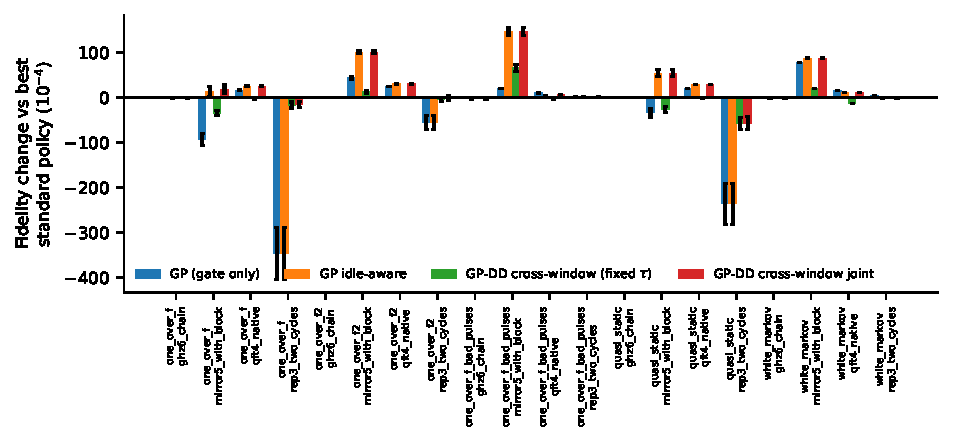
\includegraphics[width=\textwidth]{figures/novelty_c2_dd_gp.pdf}
\caption{Fidelity change against the best standard schedule per noise scenario and circuit (error bars:
two paired standard errors).}\label{fig:c2}
\end{figure*}
\begin{figure}[t]
\centering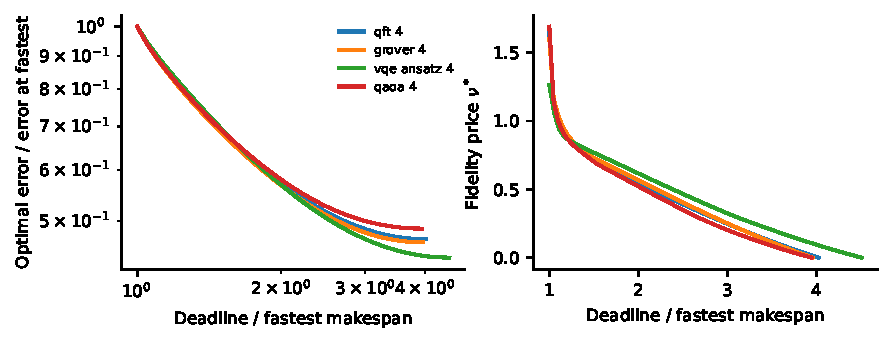
\includegraphics[width=\columnwidth]{figures/novelty_c7_frontier.pdf}
\caption{Latency--fidelity frontiers (left, log-log) and the dual fidelity price (right).}\label{fig:c7}
\end{figure}

\section{Pre-registered hardware test}
Only delays and DD pulses are controllable on current IBM Heron devices, so hardware tests target
Theorem~\ref{thm:c2} with native gate durations fixed. H1 measures CPMG decay on three qubits
($n\in\{0,2,4,8\}$, $w\in\{4,16,40,80\}\,\mu$s) and $T_1$ decay in three randomised blocks of 1{,}000 shots
($\approx$17\,s of shot time). The fitted model is frozen and the H2 circuits are hashed before submission. H2
compares no DD, XX, XY4 and GP-DD on a GHZ-5 circuit with a 20\,$\mu$s ancilla wait, in three randomised blocks of
2{,}000 shots ($\approx$7\,s). Both fit within the free tier. H2 also includes the cross-window allocation. Because simulations show that
fixed-duration GP-DD rarely beats the best standard schedule, H2 was designed as a falsification test.

\paragraph*{Calibration (H1)}
H1 ran on \texttt{ibm\_marrakesh} (qubits 55, 54, 53). It revealed strong low-frequency, partly coherent
detuning: one echo raises 16\,$\mu$s survival from 0.42 to about 0.90, and free precession revives after its first
zero crossing. Before freezing the model we therefore extended the family with a quasi-static term refocused by
any balanced block and a readout offset. We capped pulse counts at the calibrated maximum of eight per window,
because the uncapped fit would have inserted 2{,}358 pulses: pulse error cannot be identified from $n\le8$. We
also floored each qubit's pulse error at its backend-reported $X$ error. One qubit (54) is poorly described by any
model in the family.

\paragraph*{Test (H2)}
The frozen model, the circuits (hash-verified at submission) and the analysis plan were fixed before any H2 data
existed. On qubits 55, 54, 53, 39, 33, 32 at a matched 24\,$\mu$s makespan, the all-zero return probability was
0.348 for GP-DD, 0.338 for XY4, 0.321 for XX and 0.291 without DD (3 blocks $\times$ 2{,}000 shots, shot s.e.\
0.006). The pre-registered primary comparison, GP-DD minus the best standard schedule (XY4), is $+0.98$ percentage
points with shot-only 95\% interval $[-0.7, +2.7]$: \emph{not significant}, although all three blocks favour GP-DD.
The predicted ranking of all five policies matched the observed ranking exactly (Spearman 1.0). The model's
riskiest decision was to leave qubit~54 without decoupling, and that qubit's marginal survival (0.871) exceeded its
value under XY4 (0.846) and XX (0.862). GP-DD significantly outperforms Qiskit-style XX ($+2.7$ pp).

\paragraph*{Replication (R1)}
Before running it, we pre-registered an exact replication: identical hash-verified circuits, the same qubits,
4 blocks $\times$ 6{,}000 shots, and inverse-variance pooling of the two primary differences. The replication
gave GP-DD 0.326 against 0.301 for XY4, 0.296 for XX and 0.290 without DD: a difference of $+2.46$ percentage points
over XY4 (95\% interval $[+1.63, +3.29]$), with all four blocks favouring GP-DD. The pre-registered pooled
estimate is $+2.18$ points $[+1.43, +2.92]$. Qubit~54, again left undecoupled, retained a higher marginal survival
than under XY4 (0.878 vs 0.858). Absolute fidelities drifted between runs, while the two differences are
statistically consistent. All runs used one qubit chain of one device on one day, and intervals are shot-only.
Generality across chains, devices and days is therefore not established.

\section{Limitations}\label{sec:limits}
All theoretical guarantees are conditional on declared model classes. Apart from the decoupling test on one
qubit chain of one device, all results are from simulation. The single-power-law
window hazard is an approximation when quasi-static and $1/f$ noise coexist. More fundamentally, the hazard
in~\eqref{eq:window} is additive over windows, whereas low-frequency noise couples successive windows on a
qubit. For fixed schedules, the coupled hazard $c_q(\sum_k w_k(1-z_k))^{1+\beta_q}$ over binary
window-protection indicators $z_k$ is convex in $z$, separates by qubit, and is solved exactly by enumeration.
A jointly convex coupled formulation that also optimises placement and durations is open. The coverage guarantee assumes
Gaussian calibration estimates within the correct law family. Hardness for two-qubit-gate circuits is open.
Gate-duration control is not exposed on current IBM devices, so duration results remain simulation-only.
Runtime-optimal PEC offers little at long repetition delays. The anisotropic model misorders a near-tie
($<10^{-3}$) between two native-$X$ policies.

\section{Conclusion}
Geometric programming is not merely a solver for gate durations: it is the native structure of
fidelity-driven quantum resource allocation. Recognising that structure yields exact joint timing--DD
optimisation, closed-form runtime optima for mitigation, certified robustness, and sharp statements about when
optimisation cannot help. A pre-registered hardware test and its replication confirmed the model's predicted ranking
of decoupling policies, its decision to leave a noisy qubit unprotected, and a pooled 2.2-point advantage over
the best standard sequence. Testing across qubit chains, devices and days is the next step.

\appendix[Proofs]
Proofs of all statements are given in full in \texttt{docs/THEORY.md} of the accompanying repository and will be
typeset here for submission.

\bibliographystyle{IEEEtran}
\begin{thebibliography}{99}
\bibitem{kelley1961} J.~E.~Kelley, ``Critical-path planning and scheduling: Mathematical basis,'' \emph{Oper. Res.}, vol.~9, no.~3, pp.~296--320, 1961.
\bibitem{fulkerson1961} D.~R.~Fulkerson, ``A network flow computation for project cost curves,'' \emph{Manage. Sci.}, vol.~7, no.~2, pp.~167--178, 1961.
\bibitem{boyd2005} S.~Boyd, S.-J.~Kim, D.~Patil, and M.~Horowitz, ``Digital circuit optimization via geometric programming,'' \emph{Oper. Res.}, vol.~53, no.~6, pp.~899--932, 2005.
\bibitem{boyd2007} S.~Boyd, S.-J.~Kim, L.~Vandenberghe, and A.~Hassibi, ``A tutorial on geometric programming,'' \emph{Optim. Eng.}, vol.~8, no.~1, pp.~67--127, 2007.
\bibitem{jaggi2013} M.~Jaggi, ``Revisiting Frank--Wolfe: Projection-free sparse convex optimization,'' in \emph{Proc. ICML}, 2013, pp.~427--435.
\bibitem{de1997} P.~De, E.~J.~Dunne, J.~B.~Ghosh, and C.~E.~Wells, ``Complexity of the discrete time-cost tradeoff problem for project networks,'' \emph{Oper. Res.}, vol.~45, no.~2, pp.~302--306, 1997.
\bibitem{skutella1998} M.~Skutella, ``Approximation algorithms for the discrete time-cost tradeoff problem,'' \emph{Math. Oper. Res.}, vol.~23, no.~4, pp.~909--929, 1998.
\bibitem{uhrig2007} G.~S.~Uhrig, ``Keeping a quantum bit alive by optimized $\pi$-pulse sequences,'' \emph{Phys. Rev. Lett.}, vol.~98, Art.~no.~100504, 2007.
\bibitem{cywinski2008} {\L}.~Cywi\'nski, R.~M.~Lutchyn, C.~P.~Nave, and S.~Das Sarma, ``How to enhance dephasing time in superconducting qubits,'' \emph{Phys. Rev. B}, vol.~77, Art.~no.~174509, 2008.
\bibitem{biercuk2011} M.~J.~Biercuk, A.~C.~Doherty, and H.~Uys, ``Dynamical decoupling sequence construction as a filter-design problem,'' \emph{J. Phys. B}, vol.~44, Art.~no.~154002, 2011.
\bibitem{das2021} P.~Das, S.~Tannu, S.~Dangwal, and M.~Qureshi, ``ADAPT: Mitigating idling errors in qubits via adaptive dynamical decoupling,'' in \emph{Proc. MICRO}, 2021.
\bibitem{ravi2022} G.~S.~Ravi \emph{et al.}, ``VAQEM: A variational approach to quantum error mitigation,'' in \emph{Proc. HPCA}, 2022.
\bibitem{ezzell2023} N.~Ezzell, B.~Pokharel, L.~Tewala, G.~Quiroz, and D.~A.~Lidar, ``Dynamical decoupling for superconducting qubits: A performance survey,'' \emph{Phys. Rev. Appl.}, vol.~20, Art.~no.~064027, 2023.
\bibitem{temme2017} K.~Temme, S.~Bravyi, and J.~M.~Gambetta, ``Error mitigation for short-depth quantum circuits,'' \emph{Phys. Rev. Lett.}, vol.~119, Art.~no.~180509, 2017.
\bibitem{vandenberg2023} E.~van den Berg, Z.~K.~Minev, A.~Kandala, and K.~Temme, ``Probabilistic error cancellation with sparse Pauli--Lindblad models on noisy quantum processors,'' \emph{Nat. Phys.}, vol.~19, pp.~1116--1121, 2023.
\bibitem{murali2019} P.~Murali, J.~M.~Baker, A.~Javadi-Abhari, F.~T.~Chong, and M.~Martonosi, ``Noise-adaptive compiler mappings for noisy intermediate-scale quantum computers,'' in \emph{Proc. ASPLOS}, 2019, pp.~1015--1029.
\bibitem{murali2020} P.~Murali, D.~C.~McKay, M.~Martonosi, and A.~Javadi-Abhari, ``Software mitigation of crosstalk on noisy intermediate-scale quantum computers,'' in \emph{Proc. ASPLOS}, 2020, pp.~1001--1016.
\bibitem{earnest2021} N.~Earnest, C.~Tornow, and D.~J.~Egger, ``Pulse-efficient circuit transpilation for quantum applications on cross-resonance-based hardware,'' \emph{Phys. Rev. Res.}, vol.~3, Art.~no.~043088, 2021.
\bibitem{lussi2025} E.~W.~Lussi, R.~de Santiago, and E.~I.~Duzzioni, ``Time-optimization framework for the implementation of robust low-latency quantum circuits,'' \emph{Phys. Rev. Appl.}, vol.~23, Art.~no.~044036, 2025.
\bibitem{ramadan2026} Y.~A.~Ramadan, ``Quantum circuit optimization using geometric programming: Convex duration allocation on fixed NISQ circuits,'' manuscript and data, 2026. [Online]. Available: \url{https://github.com/Youssef-Ahmed38/quantum-gp-circuit-optimization}
\end{thebibliography}
\end{document}
